\documentclass[slidestop,compress,mathserif]{beamer}

\usepackage{kotex}
\usepackage{graphicx}
\usepackage{amsmath}
\usepackage{amsfonts}
\usepackage{amsthm}
\usepackage{mathrsfs}
\usepackage{setspace}
\usepackage{proof}
\usepackage{hyperref}

\title{$\lambda$Prolog로 나만의 타입체커 만들기}
\author{전남대학교 기계공학부 임기정}
\date{2021년 2월 20일}

\hypersetup{ colorlinks=true, linkcolor=blue, filecolor=magenta, urlcolor=cyan, }

\newenvironment{nemochang}
{
    \begin{center}
    \begin{tabular}{|p{0.95\textwidth}|}
    \hline
    \vspace{0.1em}
}
{
    \hline
    \end{tabular}
    \end{center}
}

\begin{document}
    \begin{frame}
        \maketitle
    \end{frame}

    \begin{frame}
        \frametitle{서론}
        \begin{itemize}
            \item 타입체커를 쉽게 만들고자 하시는 분들을 위해 발표합니다!
            \pause
            \item System-F:
            \begin{enumerate}
                \item 단순 타입 람다-계산법에 타입에 대한 보편 양화사를 추가한 시스템입니다.
                \item 하스켈과 ML 같은 함수형 언어의 이론적 기반입니다.
            \end{enumerate}
            \pause
            \item 논리형 프로그래밍:
            \begin{enumerate}
                \item \textit{규칙}이라 불리는 논리식들을 작성하는 프로그래밍 패러다임입니다.
                \item 그리하여 인터프리터가 그 규칙들로부터 질의받은 논리식을 증명할 수 있는지를 응답합니다.
            \end{enumerate}
            \pause
            \item $\lambda$Prolog:
            \begin{enumerate}
                \item 람다-식을 매칭할 수 있다는 게 가장 두드러지는 특징인 논리형 프로그래밍 언어입니다.
                \item 가장 유명한 구현체로는 Teyjus가 있는데, 본 발표에서는 \href{https://github.com/teyjus/teyjus/releases}{[링크]}에서 다운받을 수 있는 Teyjus V2를 사용할 것입니다.
            \end{enumerate}
        \end{itemize}
    \end{frame}
    
    \begin{frame}
        \frametitle{$\lambda$Prolog의 구문론}
        \begin{itemize}
            \item $\lambda$Prolog의 타입체계는 STLC에 랭크 1의 타입을 허용한 것이며, ad-hoc 다형성을 지원합니다.
            \item 변수 $x$: 하스켈과 반대로, 대문자로 시작하는 식별자입니다.
            \item 상수 $c$: 하스켈과 반대로, 소문자로 시작하는 식별자입니다.
            \item 항 $t$:
            \begin{enumerate}
                \item $t$ ::= $x$: 변수는 항입니다.
                \item $t$ ::= $c$: 상수는 항입니다.
                \item $t$ ::= $t$ $t$: 적용은 항입니다.
                \item $t$ ::= $x$\texttt{\string\ }$t$: $\lambda$-식은 항입니다.
            \end{enumerate}
            \item 원자 논리식 $A$: 타입이 $o$인 항입니다.
            \begin{enumerate}
                \item 술어: 원자 논리식 $A$의 HNF는 $ p \, t_1 \, \cdots \, t_n $ 꼴인데, 여기서 $p$를 $A$의 술어라고 합니다. 단, $n \geq 0$.
                \item 엄격한 원자 논리식 $A_r$: 술어가 상수인 원자 논리식입니다.
            \end{enumerate}
        \end{itemize}
    \end{frame}

    \begin{frame}
        \frametitle{$\lambda$Prolog의 구문론}
        \begin{itemize}
            \item 질의 $G$:
            \item $G$ ::= $A$는 규칙에 의하여 증명되는 질의입니다.
            \item $G$ ::= \texttt{true}은 항상 증명되는 질의입니다.
            \item $G$ ::= $G_1$\texttt{,} $G_2$은 $G_1$과 $G_2$ 모두를 증명해야 증명되는 질의입니다.
            \item $G$ ::= $G_1$\texttt{;} $G_2$은 $G_1$과 $G_2$ 중 하나만 증명해도 증명되는 질의입니다.
            \item $G$ ::= $D_1$ \texttt{=>} $G_2$은 $D_1$을 가정했을 때 $G_2$을 증명해야 증명되는 질의입니다.
            \item $G$ ::= \texttt{pi} $x_1$\texttt{\string\ }$G_2$은 새로운 상수 기호 $c$을 도입하여 $G_2 \left[ x_1 := c \right]$을 증명해야 증명되는 질의입니다.
            \item $G$ ::= \texttt{sigma} $x_1$\texttt{\string\ }$G_2$은 새로운 논리 변수 $X$를 도입하여 $G_2 \left[ x_1 := X \right]$를 증명해야 증명되는 질의입니다.
        \end{itemize}
    \end{frame}

    \begin{frame}
        \frametitle{$\lambda$Prolog의 구문론}
        \begin{itemize}
            \item 규칙 $D$:
            \item $D$ ::= \texttt{pi} $x_1$\texttt{\string\ }$D_2$는 머리가 $D_2$와 같은 규칙입니다.
            \item $D$ ::= $A_r$은 머리가 $A_r$인 규칙입니다.
            \item $D$ ::= $A_r$ \texttt{:-} $G$은 머리가 $A_r$인 규칙입니다.
            \item 다음과 같이 원자논리식 $p \, t_1 \, \cdots \, t_n$이 증명됩니다:
            \begin{enumerate}
                \item 머리의 술어가 $p$인 규칙을 찾습니다.
                \item $A_r$ 꼴의 규칙은 $A_r$ \texttt{:-} \texttt{true}로 볼 수 있으므로,
                \item 찾아냈다면 그 규칙을 \texttt{pi} $\bar{x}$\texttt{\string\ }($A_r$ \texttt{:-} $G$)라고 하겠습니다.
                \item 인터프리터는 새로운 논리변수 $\bar{X}$들을 도입한 뒤 $A_r \left[ \bar{x} := \bar{X} \right]$을 $p \, t_1 \, \cdots \, t_n$에 매칭시킵니다.
                \item 성공할 경우 매칭에서 발생한 치환을 $\theta$라고 할 때, $\theta \left( G \left[ \bar{x} := \bar{X} \right] \right)$의 증명을 시도합니다.
                \item 만약, 이 시도에서 실패하면, 매칭에 실패한 경우와 마찬가지로 다음 규칙을 찾습니다.
                \item 그러나, 그 시도가 성공하면, $p \, t_1 \, \cdots \, t_n$이 증명된 것입니다.
            \end{enumerate}
        \end{itemize}
    \end{frame}

    \begin{frame}
        \frametitle{시그니처}
        \begin{itemize}
            \item 이제 타입체커의 시그니처 파일을 다음과 같이 작성해봅시다.
            \begin{figure}[h]
                \begin{center}
                    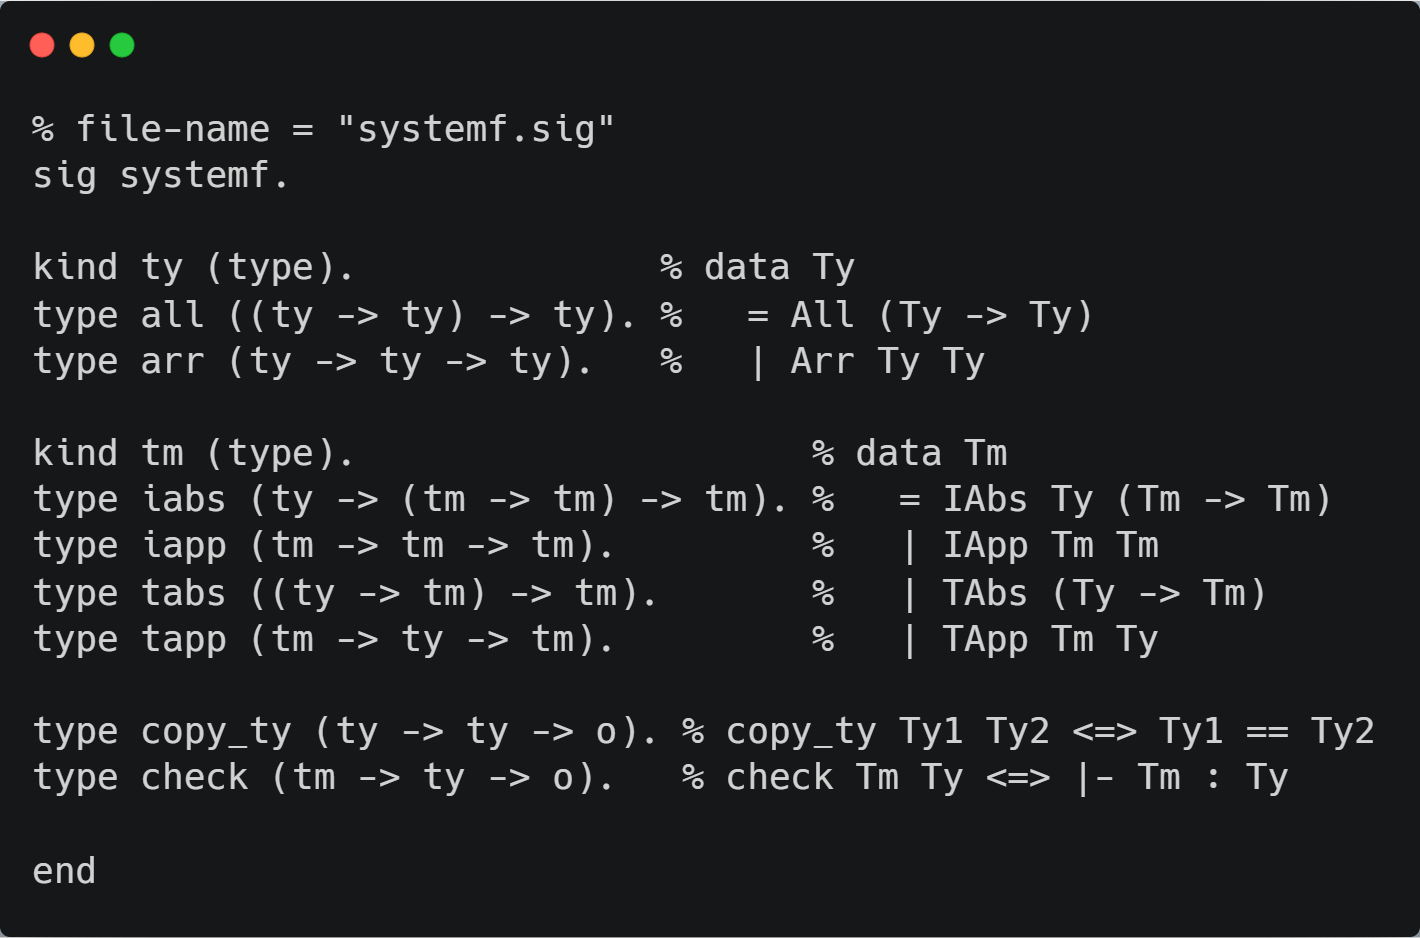
\includegraphics[width=1.0\linewidth]{sig.png}
                \end{center}
            \end{figure}
        \end{itemize}
    \end{frame}

    \begin{frame}
        \frametitle{시그니처}
        \begin{itemize}
            \item 이제부터 이 코드의 의미를 알아봅시다.
            \item 우리는 닫힌 타입과 닫힌 항만의 System-F의 타입체커를 짤 것입니다 -- 즉, 우리가 다룰 항과 타입에 자유변수가 없다고 간주합니다.
        \end{itemize}
    \end{frame}

    \begin{frame}
        \frametitle{시그니처}
        \begin{itemize}
            \item 먼저, System-F의 타입을 인코딩한 타입 생성자 \texttt{ty}에 대하여 알아봅시다.
            \item \texttt{ty}의 kind가 \texttt{*}로 선언되어 있고, 그 밑으로는 \texttt{ty}의 자료 생성자가 선언되어 있습니다.
            \item \texttt{all} ($\alpha$\texttt{\string\ }$\sigma$)는 $\left( \forall \alpha . \sigma \right)$를 인코딩한 것이며,
            \item \texttt{arr} $\tau$ $\sigma$는 $\left( \tau \to \sigma \right)$를 인코딩한 것입니다.
        \end{itemize}
    \end{frame}

    \begin{frame}
        \frametitle{시그니처}
        \begin{itemize}
            \item 그 다음, System-F의 항을 인코딩한 타입 생성자 \texttt{tm}에 대하여 알아봅시다.
            \item \texttt{tm}의 kind가 \texttt{*}로 선언되어 있고, 그 밑으로는 \texttt{tm}의 자료 생성자가 선언되어 있습니다.
            \item \texttt{iabs} $\tau$ ($x$\texttt{\string\ }$M$)은 $\left( \lambda x^{\tau} . M \right)$을 인코딩한 것입니다.
            \item \texttt{iapp} $M$ $N$은 $\left( M N \right)$을 인코딩한 것입니다.
            \item \texttt{tabs} ($\alpha$\texttt{\string\ }$M$)은 $\left( \Lambda \alpha . M \right)$을 인코딩한 것입니다.
            \item \texttt{tapp} $M$ $\tau$는 $\left( M \tau \right)$를 인코딩한 것입니다.
        \end{itemize}
    \end{frame}

    \begin{frame}
        \frametitle{시그니처}
        \begin{itemize}
            \item 마지막으로, 다음 두 술어가 선언되어 있는 게 보이네요:
            \item \texttt{copy\_ty}: 타입 \texttt{ty -> ty -> o}의 술어로서, $\sigma \left[ \alpha := \tau \right]$와 $\tau$가 주어졌을 때 가능한 ($\alpha$\texttt{\string\ }$\sigma$)를 모두 찾기 위해 필요합니다.
            \item \texttt{check}: 타입 \texttt{tm -> ty -> o}의 술어로서, $\vdash M : \sigma$일 때 그리고 그럴 때에만 \texttt{check} $M$ $\sigma$이 성립하도록 구현할 것입니다.
        \end{itemize}
    \end{frame}

    \begin{frame}
        \frametitle{구현}
        \begin{itemize}
            \item 이제 타입체커의 모듈 파일을 다음과 같이 작성해봅시다.
            \begin{figure}[h]
                \begin{center}
                    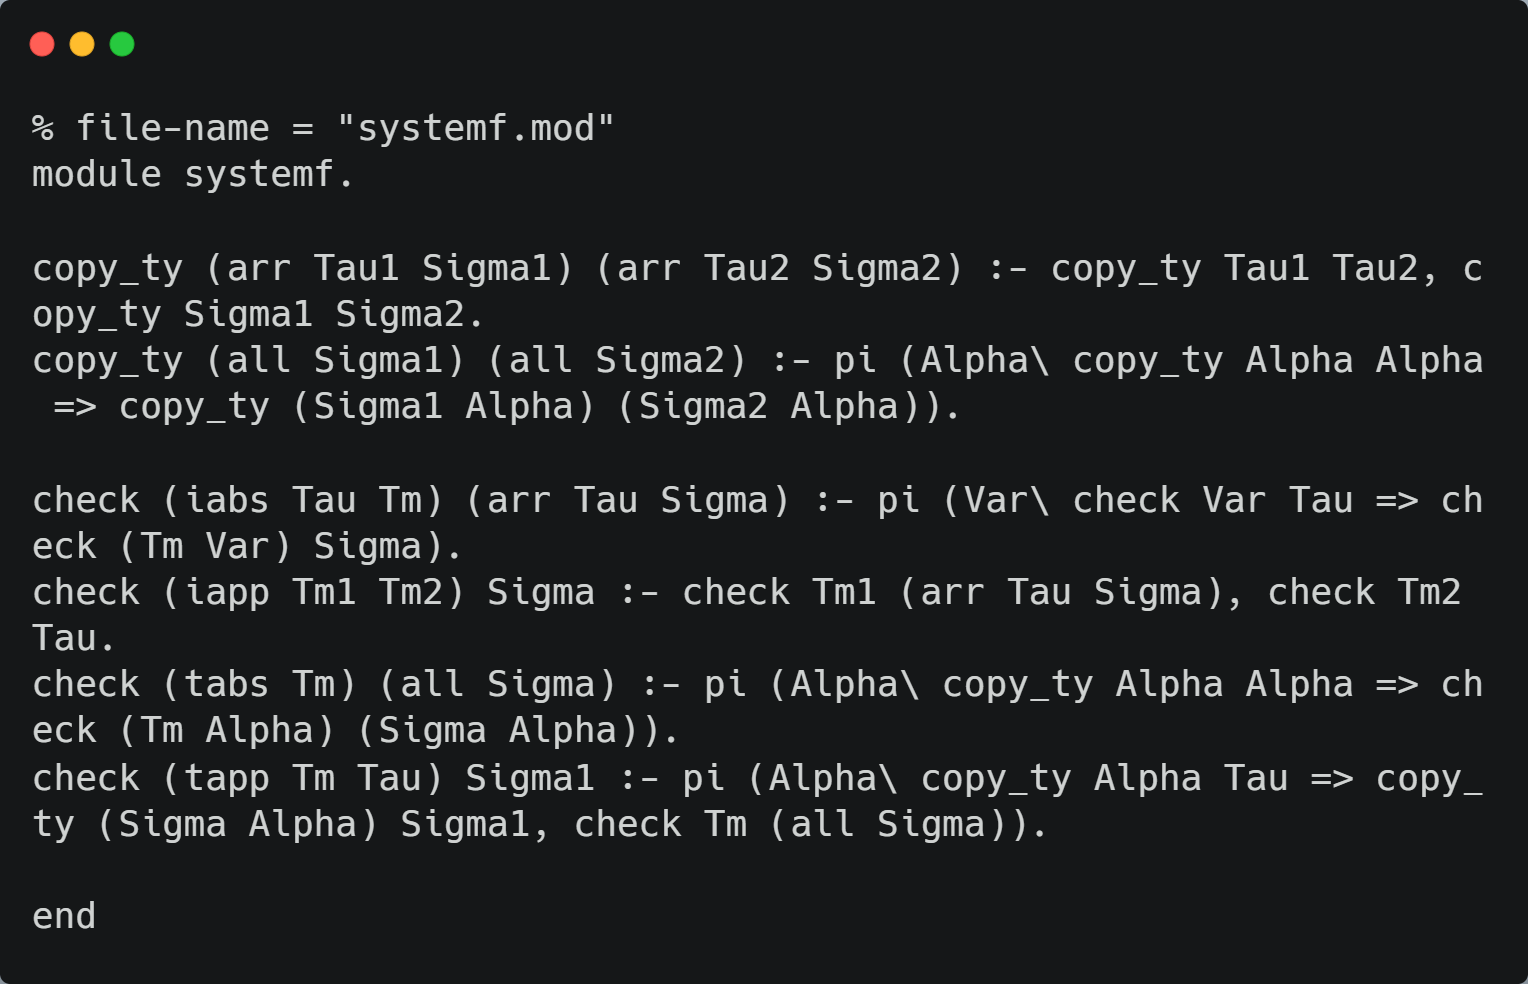
\includegraphics[width=1.0\linewidth]{mod.png}
                \end{center}
            \end{figure}
        \end{itemize}
    \end{frame}

    \begin{frame}
        \frametitle{구현}
        \begin{itemize}
            \item 먼저, \texttt{copy\_ty}의 구현부터 봅시다.
            \pause
            \item 첫 번째 규칙의 의미는 그리 어렵지 않네요:
            \begin{enumerate}
                \item $\tau_1$이 $\tau_2$의 복사본이고
                \item $\sigma_1$이 $\sigma_2$의 복사본이면,
                \item $\tau_1 \to \sigma_1$은 $\tau_2 \to \sigma_2$의 복사본이다.
            \end{enumerate}
            \pause
            \item 두 번째 규칙의 의미를 살펴봅시다:
            \begin{enumerate}
                \item 타입 \texttt{ty}의 새로운 상수 기호 $c$를 도입하고, $c$는 $c$의 복사본이라고 하자.
                \item 이때, $\tau_1 \left[ \alpha := c \right]$가 $\tau_2 \left[ \alpha := c \right]$의 복사본이면,
                \item $\forall \alpha . \tau_1$는 $\forall \alpha . \tau_2$의 복사본이다.
            \end{enumerate}
            \item 이렇게 새로운 상수 기호 $c$를 도입하는 이유는 재귀를 하기 위해 \texttt{ty -> ty}를 \texttt{ty}로 바꿔주기 위함이고,
            \item $c$는 $c$의 복사본이라는 규칙을 추가하는 이유는 재귀의 기저 단계에서 필요하기 때문입니다.
            \pause
            \item 이제 \texttt{check}의 구현을 살펴보겠습니다.
        \end{itemize}
    \end{frame}

    \begin{frame}
        \frametitle{구현}
        \begin{itemize}
            \item 첫 번째 줄을 해석하면 다음과 같습니다:
            \begin{enumerate}
                \item 타입 \texttt{tm}의 새로운 상수 기호 $c$를 도입하고, $c : \tau$라고 하자.
                \item 이때, $M \left[ x := c \right] : \sigma$이면,
                \item $\lambda x^{\tau} . M : \tau \to \sigma$이다.
            \end{enumerate}
            \item 새로운 상수 기호 $c$를 도입하는 이유는 마찬가지로 재귀하기 위해서이고,
            \item $c : \tau$라고 선언하는 이유는 역시 마찬가지로 재귀의 기저 단계에서 필요하기 때문입니다.
        \end{itemize}
    \end{frame}

    \begin{frame}
        \frametitle{구현}
        \begin{itemize}
            \item 두 번째 줄을 해석하면 다음과 같습니다:
            \begin{enumerate}
                \item $M : \tau \to \sigma$이고
                \item $N : \tau$이면,
                \item $M N : \sigma$이다.
            \end{enumerate}
        \end{itemize}
    \end{frame}

    \begin{frame}
        \frametitle{구현}
        \begin{itemize}
            \item 세 번째 줄을 해석하면 다음과 같습니다:
            \begin{enumerate}
                \item 타입 \texttt{ty}의 새로운 상수 $c$를 도입하고, $c$는 $c$의 복사본이라고 하자.
                \item 이때, $M \left[ \alpha := c \right] : \sigma \left[ \alpha := c \right]$이면,
                \item $\Lambda \alpha . M : \forall \alpha . \sigma$이다.
            \end{enumerate}
            \item $c$를 도입하는 이유는 역시 앞의 규칙들과 같습니다.
            \item $c$를 $c$의 복사본이라고 하는 이유 또한 앞에서와 마찬가지로 \texttt{copy\_ty}의 기저 단계에서 쓰기 위함입니다.
        \end{itemize}
    \end{frame}

    \begin{frame}
        \frametitle{구현}
        \begin{itemize}
            \item 네 번째 줄을 해석하면 다음과 같습니다:
            \begin{enumerate}
                \item 타입 \texttt{ty}의 새로운 상수 $c$를 도입하고, $c$를 $\tau$의 복사본이라고 하자.
                \item 이때, $\sigma \left[ \alpha := c \right]$이 $\sigma_1$의 복사본이고
                \item $M : \forall \alpha . \sigma$이면,
                \item $M \tau : \sigma_1$이다. 
            \end{enumerate}
            \item 우리는 \texttt{tapp}에 대한 타이핑 규칙을 ``$M : \forall \alpha . \sigma$이면 $M \tau : \sigma \left[ \alpha := \tau \right]$이다''라는 규칙으로 알고 있습니다.
            \item 그런데 이 규칙이 저 규칙과 같을까요? 네, 그렇습니다.
        \end{itemize}
    \end{frame}

    \begin{frame}
        \frametitle{구현}
        \begin{itemize}
            \item 먼저, 인터프리터는 $c$가 $\tau$의 복사본이라고 선언했을 때, $\sigma \left[ \alpha := c \right]$가 $\sigma_1$의 복사본이 되게 하는 $\sigma$를 찾으려고 합니다.
            \item 이때 $\sigma_1$ 안에서의 $\tau$의 나타남이
            \begin{enumerate}
                \item 기존의 \texttt{copy\_ty} 규칙에 의하여 $\tau$로 복사되어 $\sigma \left[ \alpha := c \right]$의 부분항이 되는 경우도 찾아내고,
                \item $c$가 $\tau$의 복사본이라는 규칙에 의하여 $c$로 복사되어 $\sigma \left[ \alpha := c \right]$의 부분항이 되는 경우도 찾아냅니다.
            \end{enumerate}
            \item $\sigma_1$의 나머지 부분은 \texttt{copy\_ty}에 의하여 $\sigma \left[ \alpha := c \right]$로 복사되므로,
            \item 인터프리터는 $\sigma_1 \equiv \sigma \left[ \alpha := \tau \right]$인 $\sigma$를 모두 찾아냅니다.
            \item 그 다음 인터프리터는 이렇게 얻은 모든 $\sigma$들에 대하여 $M : \forall \alpha . \sigma$인지 조사하기 때문에, 네 번째 규칙은 우리가 알고 있는 \texttt{tapp}에 대한 규칙과 결국 같은 규칙임을 알 수 있습니다.
        \end{itemize}
    \end{frame}

    \begin{frame}
        \frametitle{실행}
        \begin{itemize}
            \item 이제, 실행해 봅시다.
            \item 먼저, 컴파일러 `tjcc', 링커 `tjlink', 시뮬레이터 `tjsim'을 앞의 링크에서 다운받습니다.
            \item 그리고 다음과 같이 입력하세요:
            \begin{enumerate}
                \item \texttt{tjcc systemf}
                \item \texttt{tjlink systemf}
                \item \texttt{tjsim systemf}
            \end{enumerate}
            \item 그러면 인터프리터가 실행됩니다.
        \end{itemize}
    \end{frame}

    \begin{frame}
        \frametitle{실행}
        \begin{figure}[h]
            \begin{center}
                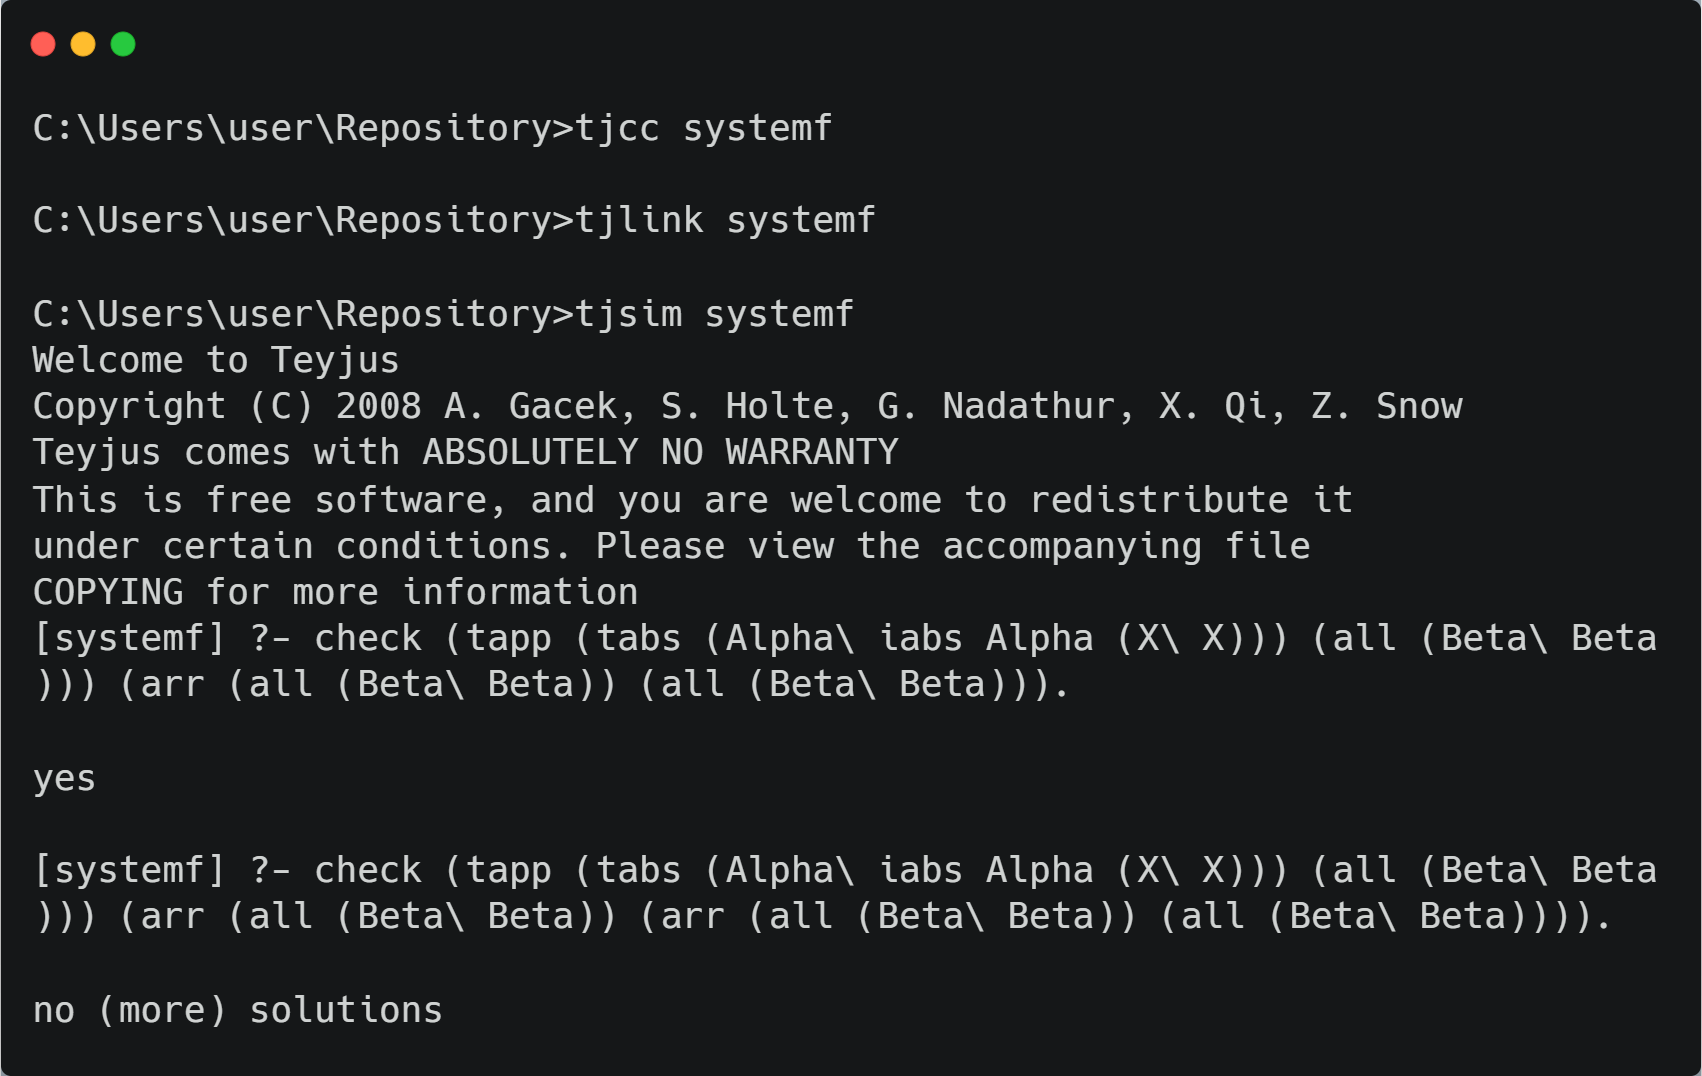
\includegraphics[width=1.0\linewidth]{fin.png}
            \end{center}
        \end{figure}
    \end{frame}

    \begin{frame}
        \frametitle{실행}
        \begin{itemize}
            \item 먼저, $$\vdash \left( \Lambda \alpha . \lambda x^{\alpha} . x \right) \left( \forall \beta . \beta \right) : \left( \forall \beta . \beta \right) \to \left( \forall \beta . \beta \right)$$인지 질의했는데,
            \item Teyjus V2는 \texttt{yes}라고 답했네요.
            \item 그 다음, $$\vdash \left( \Lambda \alpha . \lambda x^{\alpha} . x \right) \left( \forall \beta . \beta \right) : \left( \forall \beta . \beta \right) \to \left( \forall \beta . \beta \right) \to \left( \forall \beta . \beta \right)$$인지 질의했는데,
            \item Teyjus V2는 \texttt{no (more) solutions}라고 답했네요.
            \item 두 경우 모두 예상대로 작동하는 것을 알 수 있습니다.
        \end{itemize}
    \end{frame}
    
    \begin{frame}[c]
        \frametitle{끝}
        \centering
        지금까지 경청해주셔서 감사합니다!
    \end{frame}
\end{document}
